\documentclass[10pt]{article}
\usepackage[utf8]{inputenc}
\usepackage[margin=2.5cm]{geometry}

% packages die oefters gebraucht werden
\usepackage{amsmath, amssymb}
\usepackage{graphicx}
\usepackage{fancyhdr}
\usepackage{aligned-overset}

\fancyhf{}
% vspaces in den headern fuer Distanzen notwendig
% linke Seite: Namen der Abgabegruppe
\lhead{\textbf{Matthias Maile}\vspace{0.5cm}}
% rechte Seite: Modul, Gruppe, Semester
\rhead{\textbf{Höhere Mathematik II\\Sommersemester 2020}\vspace{0.5cm}}
% Center: nr. des blattes
\chead{\vspace{1.5cm}\huge{\textbf{3. Übungsblatt}}}
% benoetigt damit der eigentliche Text nicht in der Überschrift steckt
\setlength{\headheight}{3cm} 

\begin{document}
\thispagestyle{fancy}
\begin{align*}
	PI &\Leftrightarrow \text{Partielle Integration} &
	KR &\Leftrightarrow \text{Kettenregel} &
	SU &\Leftrightarrow \text{Substitution}
\end{align*}
\section*{Aufgabe 9}
\par{a) i)}
\begin{align*}
	\int_0^3 \left(e^{3x} - \sqrt[3]{e^x} \right) dx
	&= \int_0^3 \left(e^{3x} - e^{\frac x3} \right) dx \\
	% integral trennen
	&= \int_0^3 e^{3x} dx - \int_0^3 e^{\frac x3} dx \\
	% aus produktregel folgt
	&= \left[ \frac13 e^{3x} + C \right]_0^3 -
	\left[3 e^{\frac x 3} + D \right]_0^3 \\
	% einsetzen
	&= \left( \frac{e^9}{3} + C - \frac{e^0}{3} - C \right) -
	\left(3e + D - 3e^0 - D \right) \\
	% kuerzen
	&= \frac{e^9}{3} - \frac13 - 3e + 3 \\
	% alles in einen bruch
	&= \frac{e^9 - 9e +8}{3}
\end{align*}
\par{ii)}
\begin{align*}
	\int_{\frac\pi6}^{\frac\pi3} \cot(x) \ln(\sin x) dx
	&= \int_{\frac\pi6}^{\frac\pi3} 
	\frac{\cos x}{\sin x} \ln(\sin x) dx \\
	% substitution
	u := \sin(x) \Rightarrow \frac{du}{dx} = \cos(x) 
	\Rightarrow dx = \frac{du}{\cos(x)}
	\Rightarrow \
	\overset{\text{SU}}&{=}
	\int_{\sin\frac\pi6}^{\sin\frac\pi3} 
	\frac{\cos x}{\sin x} \ln(\sin x) \frac{du}{\cos x} \\
	% kuerzen
	&= \int_{\sin\frac\pi6}^{\sin\frac\pi3}
	\frac1{u} \ln(u) du \\
	% kettenregel
	\int g(x) g^\prime(x) dx \overset{KR}{=} 
	\frac12\left(g(x)\right)^2 + C
	\Rightarrow \
	&= \frac12 \left(\ln(u)\right)^2 + C 
	\vert_{\frac12}^{\frac{\sqrt{3}}{2}} \\
	% einsetzen
	&= \frac{\ln^2\left(\frac{\sqrt{3}}{2}\right) 
	- \ln^2\left(\frac12\right)}{2}
\end{align*}
\newpage
\setlength{\headheight}{0cm}
\par{b) i)}
\begin{align*}
	\int x \ln^2(x) dx 
	% partielle integration
	\overset{\text{PI, KR}}&{=} 
	\frac12 x^2 \ln^2x + C - 
	\frac12 \int x^2 * 2\ln x \frac1x dx \\
	% vereinfachen
	&= \frac12 x^2 \ln^2x + C - \int x \ln x dx \\
	% 2. partielle integration
	\overset{\text{PI}}&{=}
	\frac12 x^2 \ln^2x + C - \frac12 x^2 \ln x 
	+ \int \frac12 x^2 \frac1x dx \\
	% vereinfachen
	&=  \frac12 x^2 \ln^2x + C - \frac12 x^2 \ln x
	+ \int \frac12 x dx \\
	% integrieren
	&=  \frac12 x^2 \ln^2x  - \frac12 x^2 \ln x
	+ \frac14 x^2  + C\\
	% vereinfachen
	&= \frac12 x^2
	\left(\ln^2x - \ln x + \frac12\right) + C
\end{align*}
Da der $\ln x$ nur im Reellen nur für positive $x$ definiert ist, gilt die
eben bestimmte Stammfunktion nur für $x \in (0,\infty)$.

\vspace{0.5cm}
\par{ii)}
\begin{align*}
	\int e^{-x} \cos(5x) dx
	\overset{\text{PI}}&{=} - e^{-x} \cos(5x) + C 
	-\int e^{-x} * (-5) \sin(5x) dx \\
	% vereinfachen
	&= - e^{-x} \cos(5x) + C + 5 \int  e^{-x}\sin(5x) dx \\
	% pi
	\overset{\text{PI}}&{=}
	- e^{-x} \cos(5x) + C - 5 e^{-x} \sin(5x) 
	- 5 \int e^{-x} * 5 \cos(5x) dx \\
	% vereinfachen
	\Rightarrow
	\int e^{-x} \cos(5x) dx
	&= -e^{-x} \cos(5x) + C - 5 e^{-x} \sin(5x)
	- 25 \int e^{-x} \cos(5x) dx \qquad
	\vert + \left( 25 \int e^{-x} \cos(5x) dx \right) \\ 
	% phoenix
	\Leftrightarrow
	26 \int e^{-x} \cos(5x) dx
	&= -e^{-x} \cos(5x) + C - 5 e^{-x} \sin(5x) \\
	% kuerzen
	\Leftrightarrow
	\int e^{-x} \cos(5x) dx
	&= \frac{-e^{-x} \cos(5x) - 5 e^{-x} \sin(5x)}{26} + D
\end{align*}
Gültig für $x \in \mathbb{R}$


\section*{Aufgabe 10}
\paragraph{a)}
\par{1. Schritt:} Polynomdivision (Grad der Fkt. im Zähler $<$ Grad der 
Fkt. im Nenner)
\begin{figure}[h!]
	\centering
	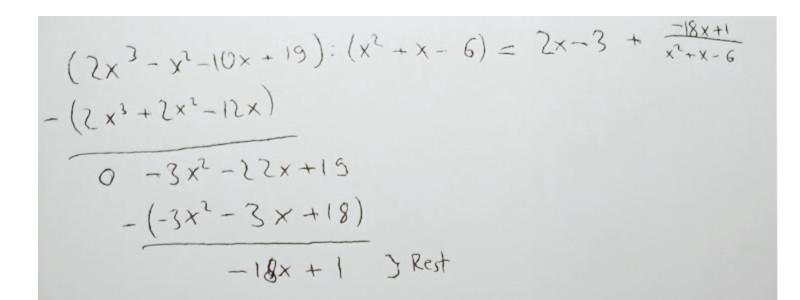
\includegraphics[width=10cm]{polynomdiv_cleaned.jpg}
\end{figure}

%
% Bild einfuegen
%
\par{2. Schritt:} Faktorisierung des Nenner-Polynoms
\[
	x^2 + x -6 = (x + 3) * (x - 2)
\]
\par{3. Schritt:} Partialbruchzerlegung
Wie nehmen dafür den Rest der Polynomdivision:
\begin{align*}
	\frac{5x + 1}{(x+3)(x-2)} 
	&= \frac{A}{x+3} + \frac{B}{x-2} \\
	\Rightarrow
	5x + 1 
	&= A * (x-2) + B * (x+3)
\end{align*}
Das liefert uns das LGS:
\begin{align*}
	A + B &= 5
	\Rightarrow A = 5-B
	\\
	-2A + 3B &= 1
	\Rightarrow -2 * (5 - B) + 3B = -10 + 5B = 1 
	\Rightarrow B = \frac{11}{5}, \ A = \frac{14}{5}
\end{align*}
Damit verbleibt das Integral:
\[
	\int \left( 2x - 3 + \frac{14}{5(x+3)} + \frac{11}{5(x-2)} \right) dx
	=
	x^2 - 3x + \frac{14}{5} \ln\vert x+3 \vert
	+ \frac{11}{5} \ln\vert x-2 \vert + C
\]

\vspace{0.5cm}
\paragraph{b)}
Grad des Polynoms im Nenner ist größer als Grad des Zählerpolynoms, ist dazu
in faktorisierter Form gegeben.\\
Partialbruch-Zerlegung:
\begin{align*}
	\frac{x}{(x-1)^3} 
	&= \frac{A}{x-1} + \frac{B}{(x-1)^2} + \frac{C}{(x-1)^3} \\
	% x-1 ^ 3 rueberbringen
	x &= A (x-1)^2 + B (x-1) + C 
	\Rightarrow A = 0 \
	^\text{$A\neq0$ impliziert ein Polynom auf der 
	rechten Seite,}
	_\text{die linke Seite ist linear}\\
	x &= Bx - B + C 
	\Rightarrow B = C = 1\\
	\Rightarrow
	\frac{x}{(x-1)^3} &= \frac{1}{(x-1)^2} + \frac{1}{(x-1)^3}
\end{align*}
Die Partialbruchzerlegung lässt sich mit der Formel 
\[
	\int \frac{1}{(x-a)^n} dx 
	= - \frac{1}{(n-1)(x-a)^{n-1}} + C
\]
integrieren:
\begin{align*}
	\int_2^5 \frac{x}{(x-1)^3} dx
	&= \int_2^5 \left( \frac{1}{(x-1)^2} + \frac{1}{(x-1)^3} \right) dx
	\\
	% auseinander ziehen
	&= \int_2^5 \frac{1}{(x-1)^2} dx 
	+ \int_2^5 \frac{1}{(x-1)^3} dx \\
	% formel benutzen
	&= \left[ -\frac{1}{
		(2-1) * (x-1)^1
	} + C \right]_2^5
	+
	\left[ -\frac{1}{(3-1) (x-1)^2} + D \right]_2^5 \\
	% vereinfachen
	&= \left[ \frac{-1}{x-1} + C \right]_2^5 +
	\left[ \frac{-1}{2 (x-1)^2} + D \right]_2^5 \\
	% einsetzen
	&= \frac{-1}{4} - \frac{-1}{1} + \frac{-1}{2 * 16} -
	\frac{-1}{2} \\
	% vereinfachen
	&= -\frac14 + 1 - \frac1{32} + \frac12 \\
	% ergebnis
	&= \frac{39}{32}
\end{align*}

\end{document}
